\documentclass[12pt]{article}
\usepackage{geometry}                % See geometry.pdf to learn the layout options. There are lots.
\geometry{letterpaper}                   % ... or a4paper or a5paper or ... 
%\geometry{landscape}                % Activate for for rotated page geometry
\usepackage[parfill]{parskip}    % Activate to begin paragraphs with an empty line rather than an indent
\usepackage{daves,fancyhdr,natbib,graphicx,dcolumn,amsmath,lastpage,url}
\usepackage{amsmath,amssymb,epstopdf,longtable}
\DeclareGraphicsRule{.tif}{png}{.png}{`convert #1 `dirname #1`/`basename #1 .tif`.png}
\pagestyle{fancy}
\lhead{CE 3354 -- Engineering Hydrology}
\rhead{SPRING 2016}
\lfoot{ES2}
\cfoot{}
\rfoot{Page \thepage\ of \pageref{LastPage}}
\renewcommand\headrulewidth{0pt}



\begin{document}
\begin{center}
{\textbf{{ CE 3354 Engineering Hydrology} \\ {Exercise Set 2}}}
\end{center}
\section*{\small{Exercises}}
\begin{enumerate}
\item Figure \ref{fig:hardinbranch.pdf} is an excerpt from the 11X17 map used in the watershed delineation workshop.  The red circle is centered on the bridge west of Eden Texas.\footnote{You will need to use the 11X17 map, the excerpt only captures a portion of the watershed that drains to the circle.  Also this watershed will be the focus of the team project, so you may wish to collectively determine the watershed for this assignment -- still will hand in individual copies.  The 11X17 pdf file is on the server if you wish to make a second copy.}

\begin{figure}[h!] %  figure placement: here, top, bottom, or page
   \centering
   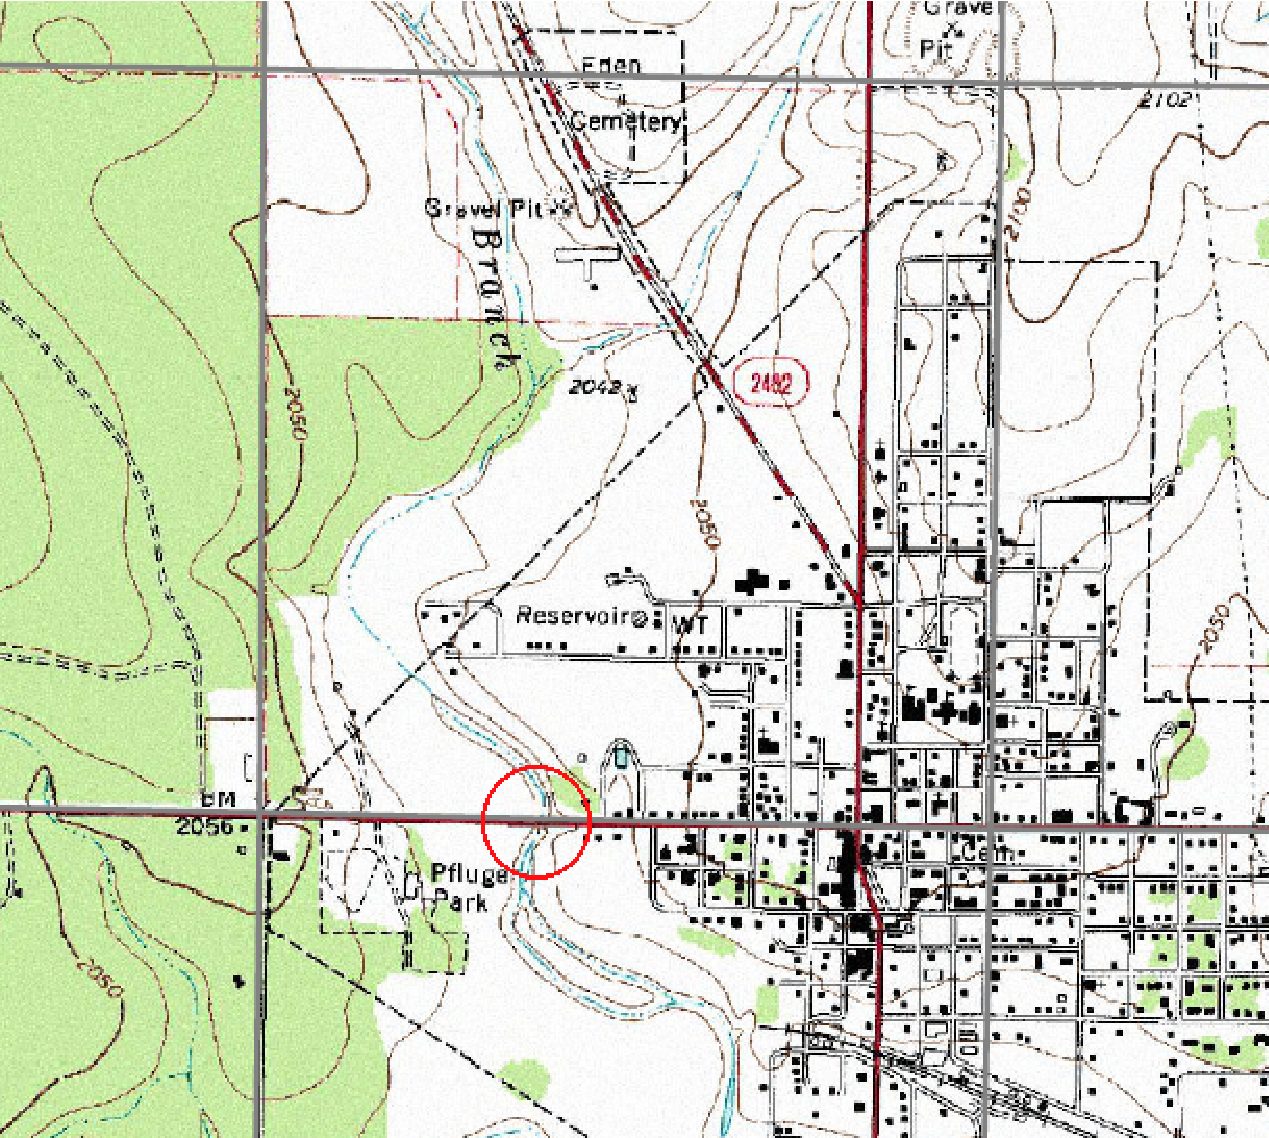
\includegraphics[width=3.5in]{hardinbranch.pdf} 
   \caption{Excerpt from 11X17 handout}
   \label{fig:hardinbranch.pdf}
\end{figure}
\clearpage

\begin{enumerate}
\item  Draw the boundary of the watershed area (delineate the watershed) that drains to the red circle. \\~\\
Figure \ref{fig:ES2-WatershedDelineated-2} shows the result of watershed delineation using a combination of a grid and topographic interpretation.   The entire system is divided into three subcatchments based on the presence of the two regulating structures (earth berms with riser pipe outlets)  

\begin{figure}[h!] %  figure placement: here, top, bottom, or page
   \centering
   \includegraphics[width=6in]{ES2-WatershedDelineated-2.jpg} 
   \caption{Study Area -- with grid overlay, outlet (Blue Dot), and subcatchments identified.  Various flow paths are indicted in transparent blue.}
   \label{fig:ES2-WatershedDelineated-2}
\end{figure}
\clearpage

\item Determine the drainage area of the watershed in square miles. \\~\\

The entire watershed area can be computed either by planimetry, or counting the squares contained within the watershed.   Each square on the figure represents an area of approximately 0.01 mi$^2$.

Figure \ref{fig:ES2-WatershedArea-2} is a scanned image of the watershed with various square counts.  The estimated area is 16.93 square miles.   This is the total drainage area including all catchments.  The sub-catchment area determinations portions are not shown on this exhibit.  

\begin{figure}[h!] %  figure placement: here, top, bottom, or page
   \centering
   \includegraphics[width=6in]{Scan.jpg} 
   \caption{Study Area -- with grid overlay, outlet (Blue Dot), and subcatchments identified.  Various flow paths are indicted in transparent blue.  1,693 Squares counted to estimate watershed area.}
   \label{fig:ES2-WatershedArea-2}
\end{figure}
\clearpage


\item Draw the main channel in the watershed (you will have to use some hydrologic judgement).  In GIS the main channel is the path from the highest elevation on the boundary to the outlet.

Figure \ref{fig:ES2-WatershedArea-3} is a scanned image of the watershed with two possible main channel paths identified.  The longer path would be selected in most instances.  For later work in the project we will need lengths of intermediate channel parts to build the hydrologic model.

\begin{figure}[h!] %  figure placement: here, top, bottom, or page
   \centering
   \includegraphics[width=6in]{Scan2.jpg} 
   \caption{Study Area -- with grid overlay, outlet (Blue Dot), and subcatchments identified.  Various flow paths are indicted in transparent blue.  1,693 Squares counted to estimate watershed area.  Two long channel paths identified.  Main channel is the longer path (assuming flow passes through the dam).}
   \label{fig:ES2-WatershedArea-3}
\end{figure}

\item Determine the length of the main channel in miles.

The main channel is about 7 miles long.

\clearpage
\end{enumerate}

\item Once your watershed is delineated, use the Web Soil Survey to estimate the soil properties on the watershed.  
As a minimum, prepare estimates of
\begin{enumerate}
\item Soil textural description (use major proportions)

Soil textural description is directly from the Web Soil Survey.
First locate the study area, then draw an outline that is reasonably close to the watershed boundary.

Figure \ref{fig:SSC-1} is a screen capture depicting the result of the process.

\begin{figure}[h!] %  figure placement: here, top, bottom, or page
   \centering
   \includegraphics[width=6in]{SoilSurveyCapture.jpg} 
   \caption{Screen capture of Web Soil Survey web page for study area.}
   \label{fig:SSC-1}
\end{figure}
\clearpage
\item Permeability/infiltration capacity (assessment of how well or poorly drained the soils are)

Soil physical properties  is directly from the Soil Data Explorer from the Web Soil Survey.

Once the study area is identified, then the data explorer can be queried to obtain physical properties data.

Figure \ref{fig:SPC-1} is a screen capture depicting the result of the process.

\begin{figure}[h!] %  figure placement: here, top, bottom, or page
   \centering
   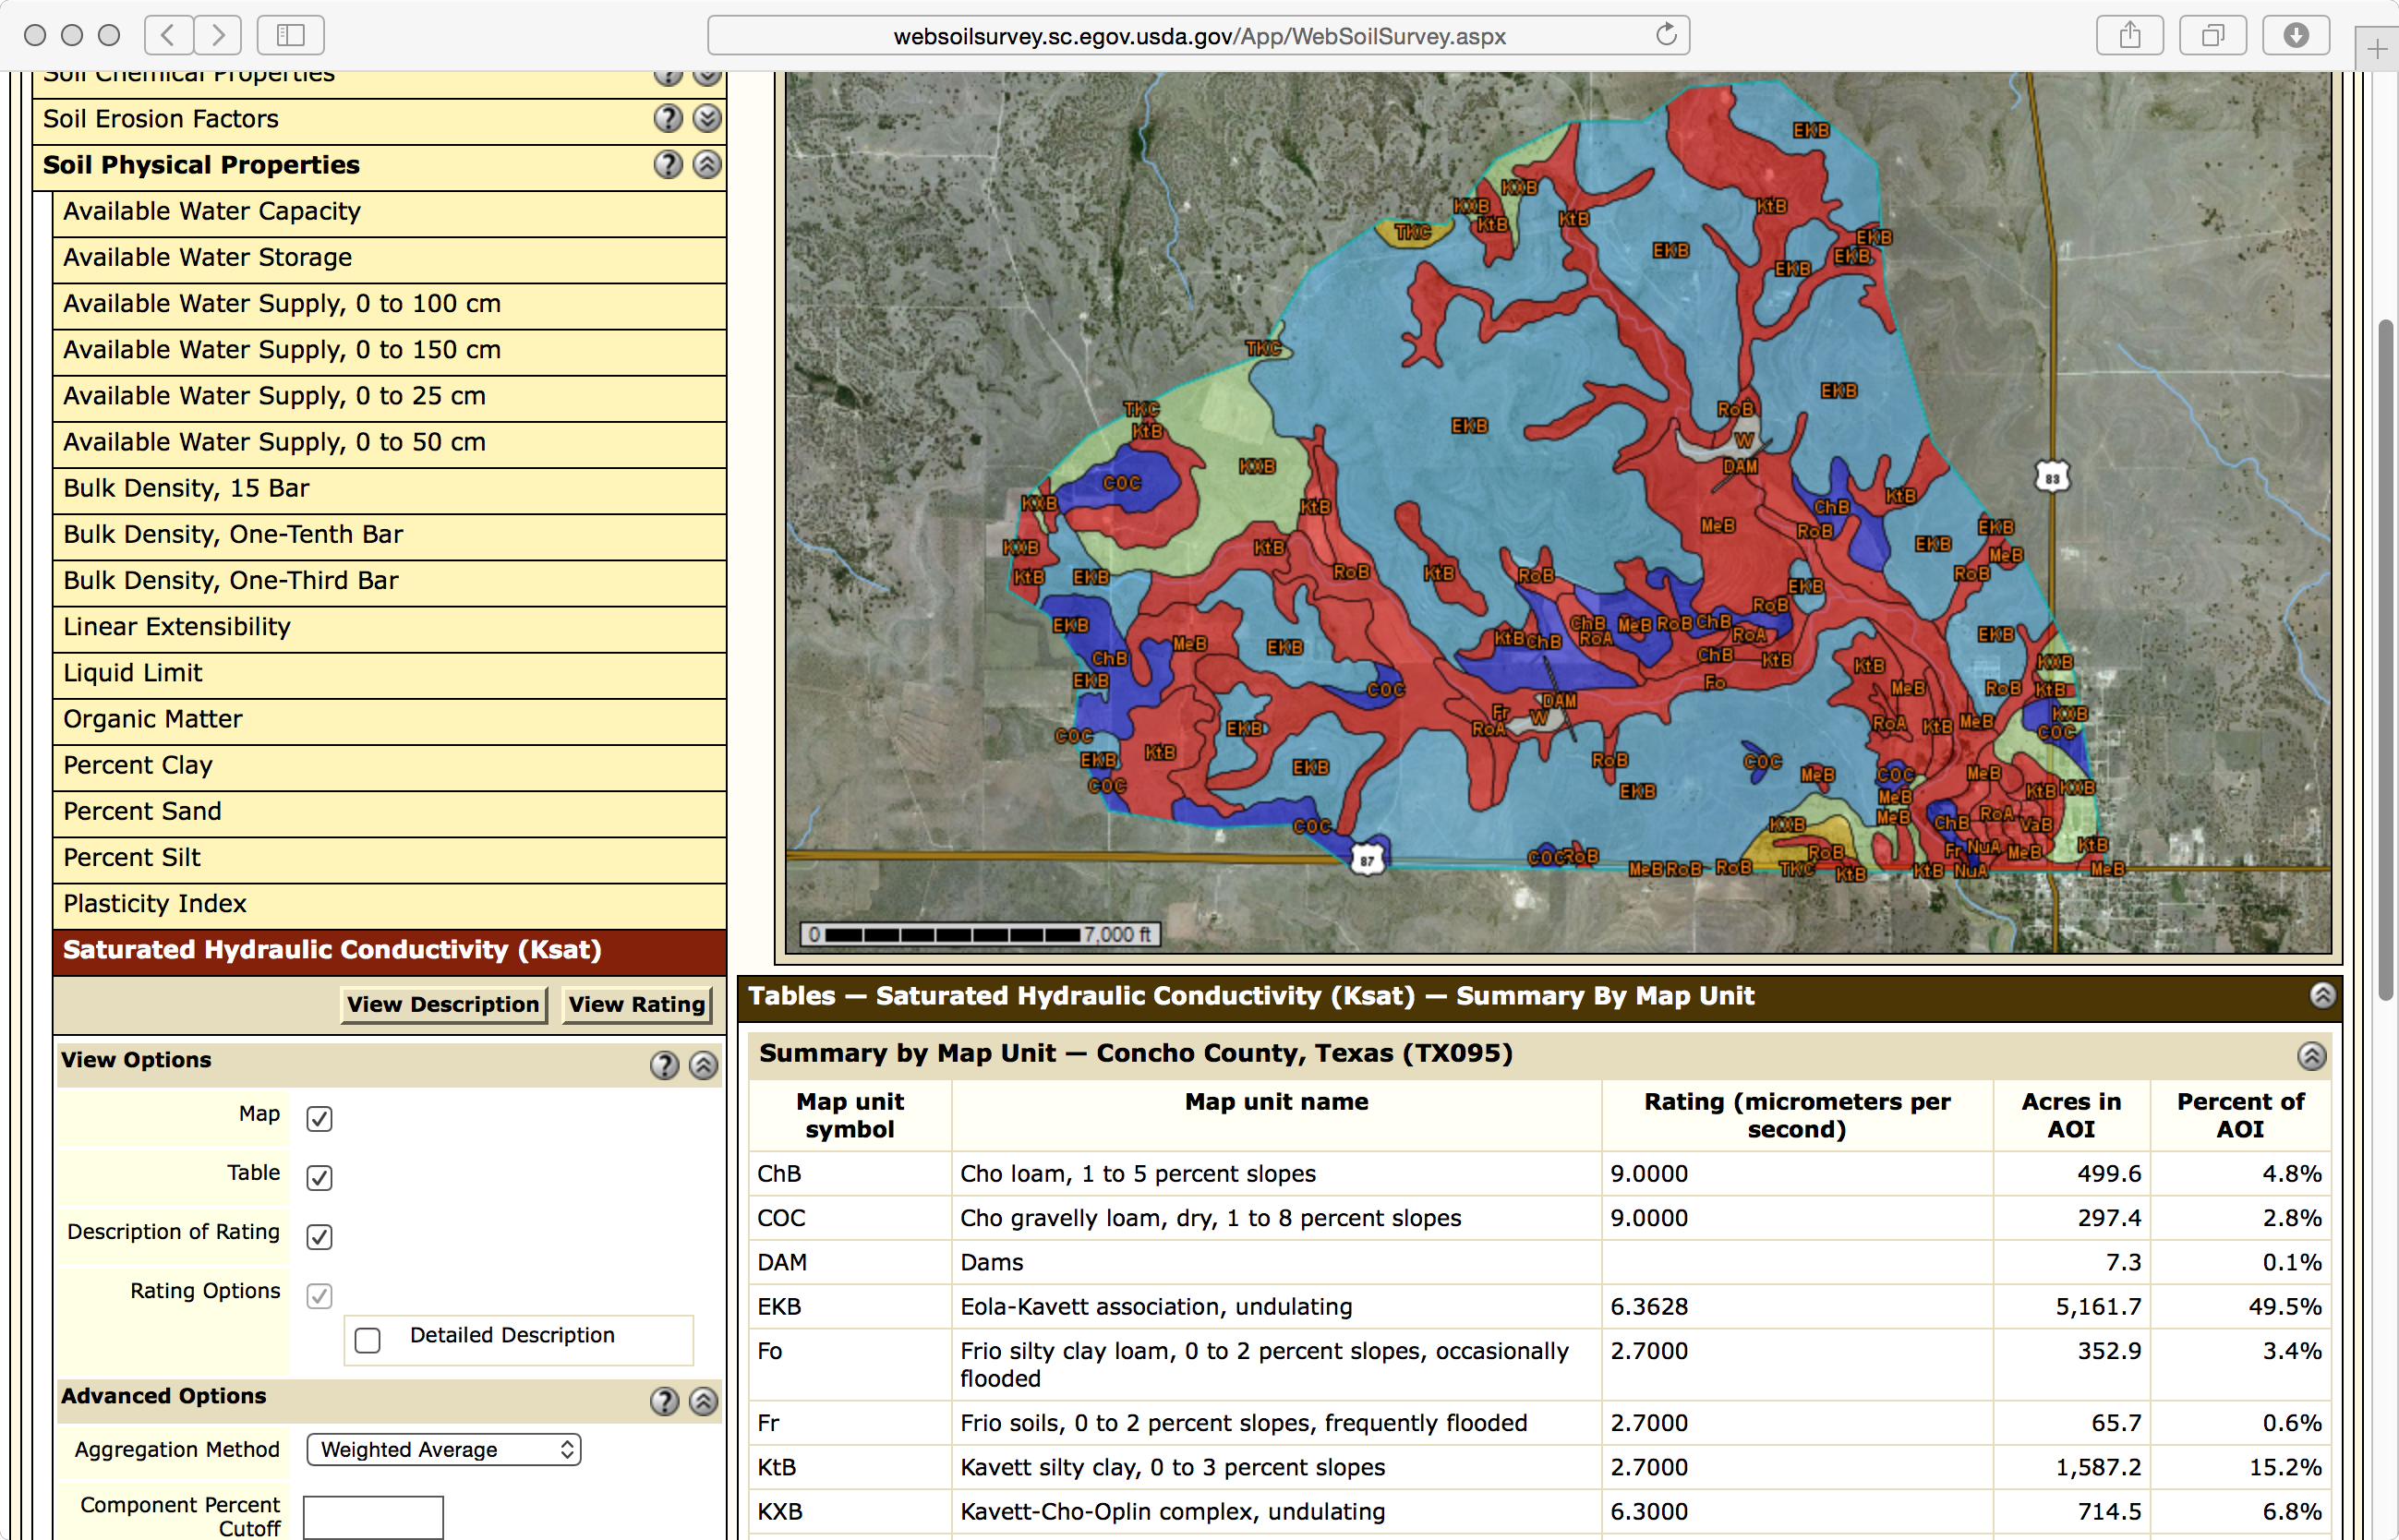
\includegraphics[width=6in]{SoilPropertyCapture.jpg} 
   \caption{Screen capture of Web Soil Survey soils properties (infiltration rates) web page for study area.}
   \label{fig:SPC-1}
\end{figure}


\end{enumerate} 
\end{enumerate}
\end{document}  